\documentclass[11pt]{article}
\usepackage[margin=1in]{geometry}
\usepackage{amsmath,amssymb}
\usepackage{algorithm}
\usepackage{algpseudocode}
\usepackage{fancyhdr}
\usepackage{enumerate}
\usepackage{graphicx}
\usepackage[colorlinks=true,linkcolor=blue,urlcolor=blue]{hyperref}

\newcommand{\hwnum}{9}

% page header, same as the posted solutions
\pagestyle{fancy}
\fancyhf{}
\lhead{EECS 376: Foundations of Computer Science\\University of Michigan, Fall 2026}
\rhead{\vspace{\baselineskip}Solutions to Homework \hwnum}
\cfoot{\thepage}
\setlength{\headheight}{28pt}

% pseudocode labels
\renewcommand{\algorithmicrequire}{\textbf{Input:}}
\renewcommand{\algorithmicensure}{\textbf{Output:}}

% notation
\newcommand{\set}[1]{\left\{#1\right\}}
\newcommand{\abs}[1]{\left|#1\right|}
\newcommand{\inner}[1]{\langle #1 \rangle}
\newcommand{\lp}{\leq_p}
\newcommand{\cproblem}[1]{\textsc{#1}}
\renewcommand{\P}{\textsf{P}}
\newcommand{\NP}{\textsf{NP}}
\newcommand{\SAT}{\cproblem{SAT}}
\newcommand{\DSAT}{\cproblem{Double-SAT}}
\newcommand{\HP}{\cproblem{HamPath}}
\newcommand{\HT}{\cproblem{HamTrek}}
\newcommand{\HC}{\cproblem{HamCycle}}
\newcommand{\AEM}{\cproblem{AffordableExactMenu}}
\newcommand{\SC}{\cproblem{Set-Cover}}
\newcommand{\NROP}{\cproblem{NROP}}
\newcommand{\OPT}{\mathrm{OPT}}
\newcommand{\ALG}{\mathrm{ALG}}
\newcommand{\qa}{q_a}
\newcommand{\qb}{q_b}
\newcommand{\win}[6]{\begin{array}{|c|c|c|}\hline #1 & #2 & #3 \\ \hline #4 & #5 & #6 \\ \hline\end{array}}

% one part per page for Gradescope
\newcommand{\qpage}[1]{\clearpage\noindent\textbf{\large #1}\par\medskip}

\begin{document}

\noindent\textbf{\large Q0 Before you start; before you submit}\par\medskip

I reviewed Handout 6 on $\NP$-hardness proofs before starting. My reductions follow its steps: describe the reduction, show it runs in polynomial time, and prove both directions of correctness.
I did not collaborate with anyone on this homework.

\qpage{Q1 Self assessment}

I chose HW8 Question 7(d), the direction $\phi \in \cproblem{3SAT} \Longrightarrow (A, s) \in \cproblem{Subset-Sum}$.
I think my proof is correct, but it could be significantly clearer and better organized.
Here is what I submitted:

\begin{center}
  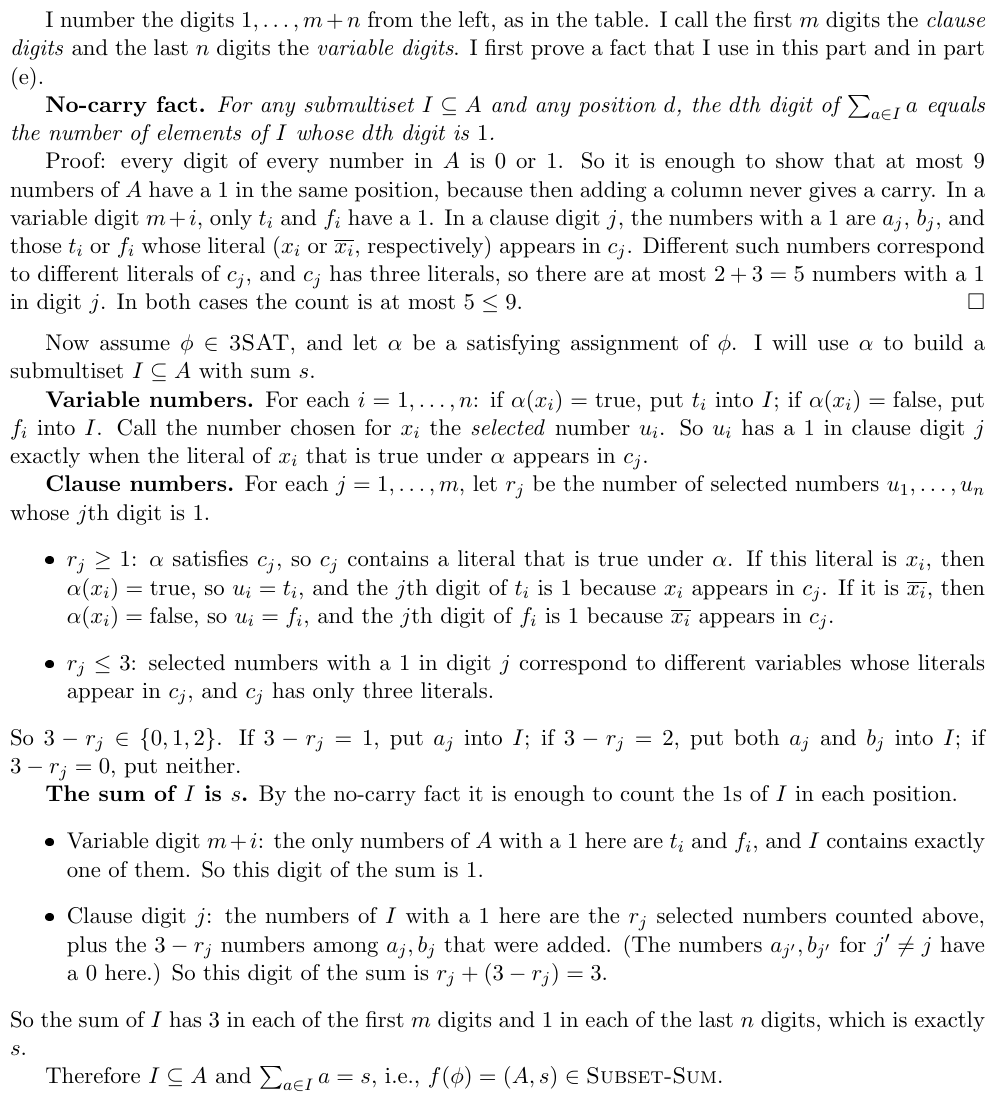
\includegraphics[width=0.62\linewidth]{hw8_q7d.png}
\end{center}

\textbf{What was deficient.}
The main idea of this direction is simple: pick $t_i$ or $f_i$ according to the satisfying assignment, so every variable digit is $1$ and every clause digit is $1$, $2$, or $3$, and then add $2$, $1$, or $0$ of $a_j, b_j$ to make each clause digit exactly $3$.
In my answer this idea is buried.
I start with a separate ``no-carry fact'' with its own proof, then I introduce extra notation (the selected numbers $u_i$ and the counts $r_j$), and the reader only sees why the sum is $s$ at the very end of the page.
The posted solution says the same thing in two short paragraphs: one for the last $n$ digits and one for the first $m$ digits.
Also, I use the no-carry fact again in part (e), but I proved it inside part (d), so part (e) depends on something hidden in another part.

\textbf{How to fix it.}
I would start with one sentence saying which subset I am going to build.
Then I would state the no-carry observation in one sentence (each column has at most $5$ ones, so adding numbers from $A$ never carries) and note that it is used again in part (e).
After that, one paragraph for the last $n$ digits (exactly one of $t_i, f_i$ is chosen, so each is $1$) and one paragraph for the first $m$ digits.
In the second paragraph I would keep the reason why each clause digit is between $1$ and $3$ before adding $a_j, b_j$ (at least $1$ because $\alpha$ satisfies $c_j$, at most $3$ because $c_j$ has three literals), since that is the step that actually uses the satisfying assignment, but I would write it in one or two sentences instead of defining $u_i$ and $r_j$.

\qpage{Q2.1 Short answers (a)}

\textbf{1. Known to be true.}
Suppose $\P \neq \NP$ and $L$ is $\NP$-complete, and assume for contradiction that $L \in \P$.
Let $A \in \NP$ be arbitrary.
Since $L$ is $\NP$-hard, $A \lp L$ by some polynomial-time function $f$.
Then $A$ is decided in polynomial time by computing $f(x)$ and running the polynomial-time decider for $L$ on $f(x)$ (the size of $f(x)$ is polynomial in $\abs{x}$, so the total time is polynomial).
So $A \in \P$ for every $A \in \NP$, i.e., $\NP \subseteq \P$.
Together with $\P \subseteq \NP$ this gives $\P = \NP$, a contradiction.
So $L \notin \P$.

\textbf{2. Unknown.}
The statement says that every language in $\NP$ is in $\P$, i.e., $\NP \subseteq \P$.
Since $\P \subseteq \NP$ is known, this is the same as $\P = \NP$.
If $\P = \NP$ the statement is true.
If $\P \neq \NP$, then by item 1 any $\NP$-complete language (for example $\SAT$) is in $\NP$ but not in $\P$, so it is a counterexample and the statement is false.
Whether $\P = \NP$ is an open problem, so the truth of the statement is unknown.

\textbf{3. Known to be true.}
Let $L$ be $\NP$-complete with $L \in \P$, and let $L'$ be any $\NP$-complete language.
Since $L' \in \NP$ and $L$ is $\NP$-hard, $L' \lp L$.
As in item 1, composing the polynomial-time reduction with the polynomial-time decider for $L$ gives a polynomial-time decider for $L'$.
So $L' \in \P$.
(In fact the same argument shows that every language in $\NP$ is in $\P$.)

\qpage{Q2.2 Short answers (b)}

An approximation algorithm always outputs a valid solution, so its value can never be better than the optimal value.

\textbf{1.} For a minimization problem, a $3/2$-approximation outputs a value $\ALG$ with $\OPT \leq \ALG \leq \frac{3}{2} \cdot \OPT$.
With $\OPT = 10$, the output is in the range
\[
  10 \leq \ALG \leq 15.
\]

\textbf{2.} For a maximization problem, a $3/5$-approximation outputs a value $\ALG$ with $\frac{3}{5} \cdot \OPT \leq \ALG \leq \OPT$.
With $\OPT = 30$, the output is in the range
\[
  18 \leq \ALG \leq 30.
\]

\qpage{Q3 The Great Ham Trek}

I show $\HP \lp \HT$.
Since $\HP$ is $\NP$-hard, this proves that $\HT$ is $\NP$-hard.
Throughout, a simple path is a path that does not repeat any vertex.

\textbf{Step 1: the reduction.}
The idea is to make every vertex other than $s$ and $t$ an event building, and require the path to visit all of them.

\begin{algorithmic}[1]
  \Require{A graph $G = (V, E)$ and vertices $s, t$}
  \Ensure{An instance of $\HT$}
  \Function{$f$}{$G, s, t$}
    \If{$s = t$ or $s \notin V$ or $t \notin V$}
      \If{$s = t$ and $V = \set{s}$} \Return $Y$ \Comment{fixed ``yes'' instance}
      \Else{} \Return $N$ \Comment{fixed ``no'' instance}
      \EndIf
    \EndIf
    \State $S \gets V \setminus \set{s, t}$
    \State $k \gets \abs{V} - 2$
    \State \Return $(G, s, t, S, k)$
  \EndFunction
\end{algorithmic}

Here $Y = (G_Y, a, b, \emptyset, 0)$ where $G_Y$ has vertices $a, b$ and the single edge $(a, b)$; it is in $\HT$ because the path $a, b$ is simple and visits $0$ vertices of $\emptyset$.
And $N = (G_N, a, b, \emptyset, 0)$ where $G_N$ has vertices $a, b$ and no edges; it is not in $\HT$ because there is no path from $a$ to $b$.
The first \textbf{if} only handles degenerate inputs: if $s \notin V$ or $t \notin V$ there is no path at all, and if $s = t$, a Hamiltonian path from $s$ to $s$ visits $s$ only once, so it has no edges and exists exactly when $V = \set{s}$.
So in these cases $f$ returns a fixed instance with the same answer.
From now on assume $s \neq t$ and $s, t \in V$, so the output is $(G, s, t, S, k)$ with $S = V \setminus \set{s, t}$ and $k = \abs{V} - 2$, which is a valid $\HT$ instance since $S \subseteq V \setminus \set{s, t}$.

\textbf{Step 2: polynomial time.}
Comparing $s$ and $t$ and checking $s, t \in V$ takes $O(\abs{V})$ time, and the fixed instances have constant size.
Copying $G$ takes $O(\abs{V} + \abs{E})$ time, building $S$ takes $O(\abs{V})$ time, and computing $k$ takes $O(\abs{V})$ time.
So $f$ runs in $O(\abs{V} + \abs{E})$ time, which is polynomial in the input size.

\textbf{Step 3a: $(G, s, t) \in \HP \Longrightarrow f(G, s, t) \in \HT$.}
Let $P$ be a Hamiltonian path from $s$ to $t$ in $G$.
$P$ visits every vertex exactly once, so it does not repeat a vertex, i.e., it is a simple path from $s$ to $t$.
$P$ visits every vertex of $S = V \setminus \set{s, t}$, so it visits exactly $\abs{S} = \abs{V} - 2 = k$ vertices of $S$.
So $(G, s, t, S, k) \in \HT$.

\textbf{Step 3b: $f(G, s, t) \in \HT \Longrightarrow (G, s, t) \in \HP$.}
Let $P$ be a simple path from $s$ to $t$ in $G$ that visits exactly $k = \abs{V} - 2$ vertices of $S$.
Since $\abs{S} = \abs{V} - 2$, $P$ visits every vertex of $S$.
$P$ also visits $s$ and $t$, its endpoints, so $P$ visits every vertex of $V = S \cup \set{s, t}$.
Since $P$ is simple, it visits each vertex at most once.
So $P$ visits each vertex exactly once, i.e., $P$ is a Hamiltonian path from $s$ to $t$, and $(G, s, t) \in \HP$.

By Steps 2, 3a, and 3b, $f$ is a polynomial-time mapping reduction, so $\HP \lp \HT$ and $\HT$ is $\NP$-hard.

\qpage{Q4.1 Cook-Levin windows (a)}

I use the convention from lecture that the state symbol is written immediately to the left of the cell the head is on.
So in the top row the head is on a $0$ with $\qa$ just before it, and after the transition the $0$ becomes $1$ and the head moves one cell to the right, so the two rows look like
\[
  \begin{array}{cccccc}
    s_1 & s_2 & \qa & 0   & s_3 & s_4 \\
    s_1 & s_2 & 1   & \qb & s_3 & s_4
  \end{array}
\]
where each $s_i \in \set{0, 1, \bot}$.
The valid windows are the following ($s_1, s_2, s_3$ each stand for any of $0, 1, \bot$).

\medskip
\textbf{Head in both rows:}
\[
  \win{s_1}{\qa}{0}{s_1}{1}{\qb}
  \qquad\qquad
  \win{\qa}{0}{s_1}{1}{\qb}{s_1}
\]

\textbf{Head in only the top row:}
\[
  \win{s_1}{s_2}{\qa}{s_1}{s_2}{1}
\]

\textbf{Head in only the bottom row:}
\[
  \win{0}{s_1}{s_2}{\qb}{s_1}{s_2}
\]

\textbf{Head in neither row:}
\[
  \win{s_1}{s_2}{s_3}{s_1}{s_2}{s_3}
\]

\qpage{Q4.2 Cook-Levin windows (b)}

To show $\SAT$ is $\NP$-hard, I need $L \lp \SAT$ for every $L \in \NP$.
Let $L \in \NP$ be arbitrary with efficient verifier $\textsc{VerifyL}$.
The statement gives a polynomial-time procedure that maps an instance $x$ of $L$ to a formula $\phi$.
This procedure is a polynomial-time mapping reduction from $L$ to $\SAT$, because
\begin{align*}
  x \in L
  &\iff \exists c \text{ such that } \textsc{VerifyL}(x, c) \text{ accepts} && \text{(definition of verifier)} \\
  &\iff \exists c \text{ such that the tableau of } \textsc{VerifyL}(x, c) \text{ has } q_{\text{accept}} \text{ in it} \\
  &\iff \phi \text{ is satisfiable} && \text{(the statement)} \\
  &\iff \phi \in \SAT.
\end{align*}
The second step holds because $\textsc{VerifyL}$ accepts exactly when it reaches $q_{\text{accept}}$, and since it runs in polynomial time (and only polynomial-size certificates matter), its whole computation fits in the polynomial-size tableau.
So $L \lp \SAT$.
Since $L \in \NP$ was arbitrary, every language in $\NP$ reduces to $\SAT$, which means $\SAT$ is $\NP$-hard.

\qpage{Q5 Search to decision}

The idea is to throw away items one at a time, keeping the removal only if a solution still exists without that item.

\begin{algorithmic}[1]
  \Require{A set $S$ of menu items with prices, and an integer $k$}
  \Ensure{At least $k$ items of $S$ with total price exactly $10k$, or ``No solution''}
  \Function{FindMenu}{$S, k$}
    \If{$D(S, k)$ rejects} \Return ``No solution''
    \EndIf
    \State $T \gets S$
    \For{each item $i \in S$}
      \If{$D(T \setminus \set{i}, k)$ accepts}
        \State $T \gets T \setminus \set{i}$
      \EndIf
    \EndFor
    \State \Return $T$
  \EndFunction
\end{algorithmic}

I say a set $X$ of items is \emph{good} if $\abs{X} \geq k$ and the total price of $X$ is exactly $10k$.
So $(X, k) \in \AEM$ if and only if $X$ has a good subset.
Note that if $X \subseteq X'$, every good subset of $X$ is also a good subset of $X'$ (the value $k$ does not change).

\textbf{Runtime.}
The algorithm calls $D$ at most $\abs{S} + 1$ times.
Every call is on an input $(T \setminus \set{i}, k)$ or $(S, k)$ with $T \subseteq S$, so each input is no larger than the original input, and since $D$ is efficient, each call takes time polynomial in the size of $(S, k)$.
Removing an item from $T$ takes $O(\abs{S})$ time.
So the total time is $\abs{S} + 1$ times a polynomial, plus $O(\abs{S}^2)$, which is polynomial in the input size.

\textbf{Correctness when there is no solution.}
If $S$ has no good subset, then $(S, k)$ is not in the language, so $D(S, k)$ rejects and the algorithm outputs ``No solution.''

\textbf{Correctness when there is a solution.}
Now suppose $S$ has a good subset, so $D(S, k)$ accepts and the algorithm continues.

\emph{Invariant: $T$ always has a good subset.}
This is true at the start since $T = S$.
$T$ only changes to $T \setminus \set{i}$ when $D(T \setminus \set{i}, k)$ accepts, i.e., when $T \setminus \set{i}$ has a good subset.
So the invariant holds after every iteration, and in particular for the final $T$.

\emph{The final $T$ is itself good.}
Let $R \subseteq T$ be a good subset of the final $T$ (it exists by the invariant).
Suppose for contradiction that $R \neq T$, and pick an item $i \in T \setminus R$.
Consider the iteration that looked at item $i$, and let $T_i$ be the value of $T$ at the start of that iteration.
Since $T$ only shrinks, $T \subseteq T_i$, so $R \subseteq T \setminus \set{i} \subseteq T_i \setminus \set{i}$.
So $R$ is a good subset of $T_i \setminus \set{i}$, which means $D(T_i \setminus \set{i}, k)$ accepted, and the algorithm removed $i$.
Items are never added back, so $i \notin T$, a contradiction.
Hence $R = T$, so $T$ is good.

So the output $T \subseteq S$ is a set of at least $k$ distinct items with total price exactly $10k$.

\qpage{Q6.1 Double-SAT (a)}

Take $\phi = x_1$.
It has exactly one satisfying assignment, $x_1 = 1$, so $\phi \in \SAT$.

The reduction outputs $\phi' = x_1 \wedge y_1$, a formula over the variables $x_1, y_1$.
$\phi'$ is true only when $x_1 = 1$ and $y_1 = 1$, so it has exactly one satisfying assignment, and $\phi' \notin \DSAT$.

So $\phi \in \SAT$ but $f(\phi) \notin \DSAT$, which breaks the condition $\phi \in \SAT \iff f(\phi) \in \DSAT$.
In general, if $\phi$ has exactly one satisfying assignment, the two copies in $\phi'$ are each forced to that assignment, so $\phi'$ also has exactly one.

\qpage{Q6.2 Double-SAT (b)}

I show $\SAT \lp \DSAT$.

\textbf{Step 1: the reduction.}
Given a Boolean formula $\phi$ over variables $x_1, \ldots, x_n$, let $z$ be a new variable that does not appear in $\phi$, and output
\[
  \phi' = \phi \wedge (z \vee \overline{z}).
\]
$\phi'$ is a Boolean formula over $x_1, \ldots, x_n, z$.
The clause $(z \vee \overline{z})$ is always true, so it does not change which values of $x_1, \ldots, x_n$ work, but it lets $z$ be either value, which doubles the number of satisfying assignments.

\textbf{Step 2: polynomial time.}
Finding a new variable name takes one pass over $\phi$ (for example, use $x_{n+1}$ where $n$ is the largest index in $\phi$), and writing $\phi'$ means copying $\phi$ and adding a constant number of symbols.
So the reduction runs in $O(\abs{\phi})$ time.

\textbf{Step 3a: $\phi \in \SAT \Longrightarrow \phi' \in \DSAT$.}
Let $\alpha$ be a satisfying assignment of $\phi$.
Define two assignments of $\phi'$: $\beta_0$ is $\alpha$ together with $z = 0$, and $\beta_1$ is $\alpha$ together with $z = 1$.
Both satisfy $\phi$, because $\phi$ does not contain $z$ and they agree with $\alpha$ on $x_1, \ldots, x_n$.
Both satisfy $(z \vee \overline{z})$, which is true for either value of $z$.
So both satisfy $\phi'$, and they are different assignments because they differ on $z$.
So $\phi'$ has at least two satisfying assignments, and $\phi' \in \DSAT$.

\textbf{Step 3b: $\phi' \in \DSAT \Longrightarrow \phi \in \SAT$.}
If $\phi'$ has at least two satisfying assignments, it has at least one, say $\beta$.
Since $\beta$ makes $\phi' = \phi \wedge (z \vee \overline{z})$ true, it makes $\phi$ true.
$\phi$ only uses $x_1, \ldots, x_n$, so the restriction of $\beta$ to $x_1, \ldots, x_n$ satisfies $\phi$.
So $\phi \in \SAT$.

By Steps 2, 3a, and 3b, $\SAT \lp \DSAT$.
Since $\SAT$ is $\NP$-hard, so is $\DSAT$.

\qpage{Q7.1 Approximate $f$-Set-Cover (a)}

First, each element is chosen at most once.
When $u$ is chosen, $A(u) \neq \emptyset$ (since $\bigcup_i S_i = U$, some $S_i$ contains $u$), and the algorithm adds $S_i$ to $C$ for every $i \in A(u)$, so $u \in C$ afterwards.
$C$ never shrinks, and Line~3 only chooses elements of $U \setminus C$, so $u$ is never chosen again.
So distinct $u, u' \in E$ are chosen in different iterations.

Now let $u, u' \in E$ be distinct, and say $u$ was chosen in an earlier iteration than $u'$.
Suppose for contradiction that there is some $i \in A(u) \cap A(u')$.
In the iteration that chose $u$, since $i \in A(u)$, the algorithm added all of $S_i$ to $C$.
Since $i \in A(u')$, we have $u' \in S_i$, so $u' \in C$ after that iteration.
$C$ never shrinks, so $u' \in C$ in the later iteration where $u'$ is chosen.
But the algorithm only chooses elements in $U \setminus C$, a contradiction.
So $A(u) \cap A(u') = \emptyset$.

\qpage{Q7.2 Approximate $f$-Set-Cover (b)}

$I_\OPT$ is a set cover, so every $u \in E \subseteq U$ is in some $S_i$ with $i \in I_\OPT$, i.e., $A(u) \cap I_\OPT \neq \emptyset$.
For each $u \in E$, pick one index $g(u) \in A(u) \cap I_\OPT$.
This defines a function $g : E \to I_\OPT$.

$g$ is one-to-one: if $g(u) = g(u')$ for distinct $u, u' \in E$, then this index is in both $A(u)$ and $A(u')$, which contradicts part (a).
Since $g$ maps $E$ one-to-one into $I_\OPT$,
\[
  \abs{E} \leq \abs{I_\OPT}.
\]

In words: each chosen element needs its own subset in any cover, because no subset contains two chosen elements.

\qpage{Q7.3 Approximate $f$-Set-Cover (c)}

\textbf{$I_\ALG$ is a set cover.}
The algorithm keeps the invariant $C = \bigcup_{i \in I} S_i$: it holds at the start ($I = C = \emptyset$), and each iteration adds $A(u)$ to $I$ and exactly the sets $S_i$ for $i \in A(u)$ to $C$.
Each iteration adds the uncovered element $u$ to $C$ (shown in part (a)), so $\abs{C}$ increases and the loop runs at most $\abs{U}$ times.
When it stops, $C = U$, so $\bigcup_{i \in I_\ALG} S_i = U$.

\textbf{$\abs{I_\ALG} \leq f \cdot \abs{E}$.}
$I$ only changes when $A(u)$ is added for a chosen $u$, so $I_\ALG = \bigcup_{u \in E} A(u)$.
Every element is in at most $f$ subsets, so $\abs{A(u)} \leq f$ for every $u$.
Hence
\[
  \abs{I_\ALG} = \abs{\bigcup_{u \in E} A(u)} \leq \sum_{u \in E} \abs{A(u)} \leq f \cdot \abs{E}.
\]

\textbf{Conclusion.}
By part (b), $\abs{E} \leq \abs{I_\OPT}$, so
\[
  \ALG = \abs{I_\ALG} \leq f \cdot \abs{E} \leq f \cdot \abs{I_\OPT} = f \cdot \OPT.
\]
The algorithm always outputs a valid set cover whose size is at most $f$ times the optimum (and it runs in polynomial time, since there are at most $\abs{U}$ iterations, each doing polynomial work).
So the $f$-cover algorithm is an $f$-approximation algorithm for $f$-$\SC$.

\qpage{Q7.4 Approximate $f$-Set-Cover (d)}

Let $f \geq 1$ be any positive integer.
Take the universe $U = \set{u}$ and $n = f$ subsets
\[
  S_1 = S_2 = \cdots = S_f = \set{u}.
\]
The element $u$ appears in exactly $f$ subsets, so this is a valid $f$-$\SC$ instance, and $\bigcup_i S_i = U$.

\textbf{$\OPT = 1$.}
$\set{1}$ is a cover since $S_1 = U$, and a cover cannot be empty since $U \neq \emptyset$.

\textbf{$\ALG = f$.}
In the first iteration $C = \emptyset$, so the only possible choice is $u$, and the algorithm adds $A(u) = \set{1, \ldots, f}$ to $I$.
Then $C = U$ and the loop ends.
So the algorithm necessarily outputs $I_\ALG = \set{1, \ldots, f}$, which has size $f$.

So on this input the algorithm's cover is exactly $f$ times as large as an optimal one.
Hence no analysis of this algorithm can give an approximation ratio better than $f$.

\qpage{Q8 (Optional extra credit) Network reliability}

The decision version is
\[
  \NROP = \set{(G, w, R, B) :
  \begin{array}{l}
    \text{there is a set } S \text{ of edges of } G \text{ with total weight at most } B\\
    \text{such that for every pair } v_i \neq v_j \text{ there are at least } R_{ij}\\
    \text{disjoint paths from } v_i \text{ to } v_j \text{ using only edges in } S
  \end{array}}.
\]
Here disjoint paths are distinct paths that share no vertex except their endpoints.

I show that $\HC \lp \NROP$, where $\HC$ is the Hamiltonian cycle problem from lecture.

\textbf{Step 1: the reduction.}
Given an undirected graph $G = (V, E)$ with $n = \abs{V}$ vertices:
if $n \leq 2$, output a fixed ``no'' instance of $\NROP$ (a simple graph with at most $2$ vertices has no Hamiltonian cycle; for example, two vertices with no edges, $R_{12} = 1$, $B = 0$).
Otherwise output $(G, w, R, B)$ with $w(e) = 1$ for every edge, $R_{ij} = 2$ for all $i \neq j$ ($R_{ii} = 0$), and $B = n$.

\textbf{Step 2: polynomial time.}
Setting the weights takes $O(\abs{E})$ time, writing $R$ takes $O(n^2)$ time, and $B$ takes $O(\log n)$ bits.
So the reduction runs in $O(n^2 + \abs{E})$ time.

\textbf{Step 3a: $G \in \HC \Longrightarrow$ output $\in \NROP$.}
Let $H$ be a Hamiltonian cycle of $G$ and let $S$ be its $n$ edges, so the weight of $S$ is $n = B$.
For any two distinct vertices $v_i, v_j$, removing them splits the cycle $H$ into two arcs, which give two paths from $v_i$ to $v_j$ using only edges of $S$.
They share no vertex except $v_i$ and $v_j$, and they are different paths (since $n \geq 3$, at least one arc has an internal vertex).
So there are $2 = R_{ij}$ disjoint paths for every pair, and the output is in $\NROP$.

\textbf{Step 3b: output $\in \NROP \Longrightarrow G \in \HC$.}
Let $S \subseteq E$ have weight at most $B = n$, i.e., $\abs{S} \leq n$, with $2$ disjoint paths in $S$ between every pair of vertices.

\emph{Every vertex has degree at least $2$ in $S$.}
Take any vertex $v$ and any other vertex $u$.
There are two disjoint paths $P_1, P_2$ from $v$ to $u$ in $S$.
If they started with the same edge $(v, x)$: when $x \neq u$, $x$ would be a shared vertex other than the endpoints; when $x = u$, both paths would be the single edge $(v, u)$, so they would be the same path.
Both are impossible, so $P_1$ and $P_2$ start with different edges at $v$, and $v$ has degree at least $2$ in $S$.

\emph{$S$ is a Hamiltonian cycle.}
The degrees add up to $2\abs{S} \leq 2n$, and each of the $n$ vertices has degree at least $2$, so every vertex has degree exactly $2$ in $S$.
A graph in which every vertex has degree $2$ is a union of disjoint cycles.
$S$ connects every pair of vertices (there is at least one path), so it is a single cycle, and this cycle passes through all $n$ vertices.
Since $S \subseteq E$, it is a Hamiltonian cycle of $G$, so $G \in \HC$.

(For $n \leq 2$, $G \notin \HC$ and the fixed output is not in $\NROP$, since with $B = 0$ no edge can be used, so the two vertices have no path.)

By Steps 2, 3a, and 3b, $\HC \lp \NROP$.
Since $\HC$ is $\NP$-hard, the decision version of $\NROP$ is $\NP$-hard.

\end{document}
